\documentclass[output=paper]{langsci/langscibook} 
\ChapterDOI{10.5281/zenodo.2583814}
\author{Karsten Schmidtke-Bode\affiliation{Leipzig University and Friedrich Schiller University Jena}}
\title{Attractor states and diachronic change in Hawkins’s “Processing Typology”}
\abstract{This paper provides an assessment of John Hawkins's (\citeyear{Hawkins2004_Eff,Hawkins2014_VarEff}) programme of explaining cross-linguistic regularities in terms of functional-adaptive principles of efficient\is{efficiency} information processing. In the first part of the paper, I systematize how such principles may possibly affect the diachronic development of languages, and I argue that evidence for efficient\is{efficiency} coding can be obtained primarily from the actualization process, rather than the innovation stage that is at the focus of purely source-based approaches to explaining universals. In the second part of the paper, I present a small case study on a specific prediction made in \citet{Hawkins2014_VarEff}, concerning the typology and diachrony of \isi{article} morphemes. This will allow us to carve out both strengths and weaknesses of Hawkins’s programme in its current manifestation.
}
% %% hyphenation points for line breaks
%% Normally, automatic hyphenation in LaTeX is very good
%% If a word is mis-hyphenated, add it to this file
%%
%% add information to TeX file before \begin{document} with:
%% %% hyphenation points for line breaks
%% Normally, automatic hyphenation in LaTeX is very good
%% If a word is mis-hyphenated, add it to this file
%%
%% add information to TeX file before \begin{document} with:
%% %% hyphenation points for line breaks
%% Normally, automatic hyphenation in LaTeX is very good
%% If a word is mis-hyphenated, add it to this file
%%
%% add information to TeX file before \begin{document} with:
%% \include{localhyphenation}
\hyphenation{
affri-ca-te
affri-ca-tes
com-ple-ments
Haw-kins
broad-er
over-view
par-tic-u-lar
spe-cif-ic
adap-tive
lin-guis-ti-cal-ly
Hix-kar-yana
sour-ces
mark-er
ground-ed
evol-ved
Born-kessel-Schlesew-sky
}
\hyphenation{
affri-ca-te
affri-ca-tes
com-ple-ments
Haw-kins
broad-er
over-view
par-tic-u-lar
spe-cif-ic
adap-tive
lin-guis-ti-cal-ly
Hix-kar-yana
sour-ces
mark-er
ground-ed
evol-ved
Born-kessel-Schlesew-sky
}
\hyphenation{
affri-ca-te
affri-ca-tes
com-ple-ments
Haw-kins
broad-er
over-view
par-tic-u-lar
spe-cif-ic
adap-tive
lin-guis-ti-cal-ly
Hix-kar-yana
sour-ces
mark-er
ground-ed
evol-ved
Born-kessel-Schlesew-sky
}
\begin{document}
\maketitle 
 
\section{Introduction} 

In debating the role of source- and result-oriented explanations in typology, a research programme that merits discussion is John Hawkins’s approach to cross-linguistic variation, laid out most comprehensively in Hawkins (\citeyear{Hawkins1994_Perf,Hawkins2004_Eff,Hawkins2014_VarEff}). The overarching hypothesis of these works is that many cross-linguistic generalizations about grammatical structure can be explained as adaptations\is{adaptation} to efficient\is{efficiency} information \isi{processing} (“\isi{processing} typology”, see \citealt{Hawkins2007_Proc}). In a nutshell, Hawkins argues that efficient\is{efficiency} information \isi{processing} can be achieved by (i) “minimizing domains” in which certain semantic and syntactic relations are processed, (ii) “minimizing forms” whenever their information content is recoverable from the context or long-term statistical knowledge, (iii) arranging elements in such a way that the ultimate message can be transmitted as rapidly and accurately as possible, i.e. without delays, false predictions, backtracking, etc. These \isi{efficiency} principles are thus \isi{attractor}s that are assumed to affect linguistic choices in usage events and ultimately also the conventionalized shapes of grammars.

Hawkins’s programme is one of the most systematic attempts to ground typological data in \isi{psycholinguistic} research and to link it to the arena of language use; in this spirit, it is similar, for example, to the work of Bybee (\citeyear{Bybee1985_Morph,Bybee2010_Cogn}) and Croft (\citeyear{Croft2001_RadCon,Croft2003_Typ}). Moreover, Hawkins’s “performance-grammar-correspondence hypothesis”, according to which grammatical rules are basically crystallized usage preferences, echoes one of the key tenets of the usage-based theory\is{usage-based approach} of language (\citealt{Langacker1987_Found,Kemmer2000_Intro}). And some specific \isi{efficiency} principles, such as the “minimization of forms” in proportion to their degree of \isi{predictability}, even have exact parallels in other functional-typological works (e.g. \citealt{Haiman1983_Icon,Croft2003_Typ,Haspelmath2008_Econ}). 

At the same time, however, Hawkins’s work is not always received uncritically within usage-based linguistics\is{usage-based approach}. Among other things, it is couched in a formal phrase-structure architecture that appears to presuppose the existence of many grammatical categories (see \citealt{Diessel2016_Corr}); some of its principles have been criticized for not being truly domain-general but perhaps specific to language (such as a pressure for short constituent recognition domains, see \citealt{Bybee2010_Cogn}); and crucially in the present context, Hawkins has also been criticized for neglecting or underestimating the diachronic dimension behind the phenomena he attempts to explain (e.g. \citealt{Cristofaro2017_Dep}; \citealtv{Collins2019tv}). But to the extent that Hawkins does make reference to historical developments, the nature and plausibility of his diachronic claims are worth investigating in more detail, which is precisely what the present contribution aims to do. 

To this end, the first part of the paper develops a systematization, in the usage-based framework\is{usage-based approach}, of how Hawkins’s functional-adaptive\is{adaptation} principles possibly affect the diachronic development of languages. I argue that there is solid evidence for efficient\is{efficiency} information \isi{processing} in the moulding of grammar, suggesting that there is a place for result-oriented processes, beside source determination, in accounting for typological distributions. In the second part of the paper, I exemplarily focus on a diachronic prediction made in \citet{Hawkins2014_VarEff}, according to which languages of different word-order\is{word order} types show markedly different propensities for grammaticalizing\is{grammaticalization} definite\is{definiteness} \isi{article}s (the prediction will be formulated more precisely as we go along). This miniature case study will not only serve as a testing ground for this specific \isi{efficiency}-based hypothesis, but also allow us to identify some general merits and potential problems of \isi{processing} typology.

\section{The diachronic dimension in processing typology} 

In the \isi{usage-based approach}, language change is conceived as a multi-step process (\citealt{Croft2000_Change,Croft2006_Change,Aitchison2013_Change}) that starts by breaking a convention in the form of a linguistic \isi{innovation} (“altered replication”), followed by the spread of that \isi{innovation} through both the linguistic system (“\isi{diffusion}”) and the speech community (“\isi{propagation}”). Hawkins’s publications contain a number of indications as to how his \isi{efficiency} principles influence \isi{innovation}, \isi{diffusion} and \isi{propagation} processes. I will tackle each of them briefly, in reverse order, as this reflects an increasing degree of explicitness of the respective proposals.\footnote{Although the present section is specifically about Hawkins’s work, it actually applies to “functional-adaptive\is{adaptation} constraints” (\citealtv{Haspelmath2019tv}) more generally, not least because Hawkins’s \isi{processing} typology draws on and incorporates similarly-minded principles from many other functionalist typologists (e.g. \ia{Greenberg}, \ia{Comrie}, \ia{Keenan}, \ia{Givón}, \ia{Haiman}, \ia{Croft}, \ia{Haspelmath}, etc.).}

As for \isi{propagation} processes, \ia{Hawkins} is usually reticent with regard to the forces that implement efficient\is{efficiency} structures, even though the central diachronic mechanism in his programme is that of “\isi{selection}”: Efficient\is{efficiency} variants are said to be selected\is{selection} relatively more frequently\is{frequency} than their inefficient\is{efficiency} counterparts, until they may ultimately oust the inefficient\is{efficiency} ones completely. It is in this way, Hawkins argues, that preferred patterns in performance can conventionalize into grammatical rules, although he concedes in \citet[10]{Hawkins2014_VarEff} that it is presently poorly understood how exactly this “translation from performance to grammar” works. Now, if one subscribes to the view that \isi{propagation} is entirely driven by sociolinguistic forces like prestige, solidarity and the resulting \isi{accommodation} (e.g. \citealt{Croft2000_Change}; \citealt{Cristofaro2017_Dep}; \citealtv{Cristofaro2019tv}), it remains mysterious, indeed, how Hawkins’s very idea of \isi{selection} processes can fit in. 

On the other hand, there are well-known accounts of language change in which \isi{propagation} is not exclusively a social phenomenon: \citegen{Keller1994_Invis} “\isi{Invisible Hand}” theory, for example, leaves room for functional considerations in the \isi{selection} process. Some of Keller’s classic examples of invisible-hand processes, such as the emergence of a traffic jam or a short-cutting footpath do not, in fact, involve social motives: People follow a certain course of action because they primarily consider its functional advantages, regardless of the sociolinguistic profile of the person whose behaviour they adopt. \citet{Cristofaro2017_Dep} claims that there is no empirical evidence at all for this scenario in linguistics, but this assessment is overly pessimistic: \citet{Rosenbach2008_Change}, in a detailed examination of \isi{evolution}ary accounts of language change, concludes that “the evidence available does not speak for the \textit{exclusive} role of social factors in the \isi{selection} process” (\citealt{Rosenbach2008_Change}: 44; emphasis in original). Therefore, I currently see no reason to dismiss a priori a theory in which both social and functional \isi{selection} pressures can be operative in \isi{propagation} (see also \citealt{Haspelmath1999_Opt,Nettle1999_Div,Enfield2014_Caus} for similar positions).\footnote{Note that recent mathematical models of language change (e.g. \citealt{BlytheCroft2012}) clearly show that \isi{selection} as such is a crucial element of \isi{propagation} processes, in as far as alternative models of \isi{propagation} that do not rely on a weighting of linguistic variants (e.g. \citealt{Trudgill2004_Dial}) do not produce the empirical patterns of \isi{propagation} that have been established in historical linguistics and sociolinguistics. However, \citet{BlytheCroft2012} also concede that their model cannot distinguish between social and functional factors in \isi{selection}, i.e. it leaves open which of these is more vital in the \isi{propagation} process or how they possibly interact.} On this view, then, Hawkins’s \isi{efficiency} principles are relevant to, and hence at least partially drive, the \isi{propagation} process, although empirical evidence that clearly disentangles functional and social \isi{selection} processes is, of course, very hard to come by (see also \citealt{Seiler2006_Func}). 

The empirical picture is clearer, in my view, when it comes to \textsc{\isi{diffusion}} or \textsc{\isi{actualization}} processes, i.e. the spread of an \isi{innovation} through the linguistic system.\footnote{The term \textsc{\isi{diffusion}} is best-known in the context of “lexical \isi{diffusion}” \citep{Wang1969_Diff}, which refers to the successive spread of a phonetic or morphosyntactic \isi{innovation} to different lexical items (e.g. the Progressive\is{progressive} construction to more and more lexical verbs, or final consonant \isi{devoicing} to all relevant words). In the present paper, I am using the term \isi{diffusion} in a broader sense, comprising also the application of an innovated grammatical marker or construction to a new morphosyntactic environment (e.g. the extension\is{analogy} of \textit{all but} in its historically younger sense ‘almost’ from adjectival\is{adjective} uses (\textit{This was all but remarkable}) to verbal environments (\textit{He all but fell down}), see  \citealt{DeSmet2012_Act}). Diffusion\is{diffusion} is thus synonymous with the term \textsc{\isi{actualization}} (\citealt{Timberlake1977_Act}, \citealt{Andersen2001_Actual} and many others, most recently  \citealt{DeSmet2012_Act}).} Although Hawkins himself does not speak of \isi{diffusion} or \isi{actualization}, the process is actually highly germane to his research, as many of the phenomena he discusses in support of his \isi{efficiency} theory are cases of limited \isi{diffusion}. In relativization\is{relative clause}, for example, a well-known pattern is for resumptive \isi{pronoun}s, once they have been innovated, not to spread across the entire range of relativization\is{relative clause} sites, but to be restricted to certain sections of \citegen{KeenanComrie1977} \isi{accessibility hierarchy} (as in \ili{Hausa}, \ili{Hebrew}, \ili{Welsh} and many other languages). Similarly, when \isi{object} \isi{case} markers develop and spread within the linguistic system, they typically end up being confined to animate\is{animacy}, definite\is{definiteness} or pronominal\is{pronoun} \isi{object}s, rather than being extended across the board (see, e.g., \citealt{Sinnemäki2014} for a quantitative study). 

Many other cases of such differential marking are collected in \citet{Haspelmath2008_Econ} and subsumed by \citet{Hawkins2004_Eff,Hawkins2014_VarEff} under his “Minimize Forms” principle: The marker in question is applied to those environments that require more \isi{processing} effort, and is left out economically\is{economy} elsewhere. Processing\is{processing} effort, in turn, may be related to various factors, notably constraints on working memory (e.g. longer \isi{processing} domains correlating with resumptive \isi{pronoun}s) and the relative unexpectedness (‘\isi{surprisal}’) of a given configuration (see \citealt{NorcliffeEtAl2015} on memory- and expectation-based \isi{processing} in cross-linguistic perspective). For example, discourse participants and animate\is{animacy} entities are more likely to be \isi{subject}s than \isi{object}s, hence it is precisely these kinds of \isi{object}s that are more surprising\is{surprisal}. Paired with the Hawkinsian\ia{Hawkins} assumption of \isi{efficiency} on the part of the speaker, it is also only these \isi{object}s that need to be marked overtly. A similar \isi{surprisal}-based account is provided by \citet{Haig2018_DOI} to explain “why differential object\is{differential object marking} \isi{indexing} is an \isi{attractor} state” \citep[781]{Haig2018_DOI} in the \isi{grammaticalization} of \isi{object} \isi{pronoun}s.

In Hawkins’s programme, then, all of these cases are amenable to an explanation in terms of efficient\is{efficiency} information \isi{processing}. I believe that this account is presently superior to purely source-oriented typologies such as \ia{Cristofaro}’s, for the following reasons.

Firstly, there is solid evidence for \isi{efficiency} where the occurrence of a particular marker is optional. This can be observed, for example, with variable relativizers\is{subordinator} that, other things being equal, show up less frequently\is{frequency} when a \isi{relative clause} is statistically expected given the previous co-text, and vice versa (\citealt{WasowEtAl2011}). As \citet{FoxThompson2007} observe, a sentence like

\ea
{\textit{This was the ugliest set of shoes} [\textit{I ever saw in my life}].} \\
\z

\noindent would sound “quite awkward” (\citealt{WasowEtAl2011}: 181) if the \isi{relative clause} were introduced by \textit{that}; according to Wasow et al., this is precisely because a \isi{relative clause} is expected in this context, which is in turn why relative \textit{that} tends to be omitted efficiently\is{efficiency}. \citet{Jaeger2010_Red} shows that similar \isi{predictability} effects account for a large portion of the variability of the \ili{English} \isi{complementizer} \textit{that}. 

Importantly, the same kinds of effect also show up in \isi{psycholinguistic} experimentation, and in languages other than \ili{English}. For example, recent studies have shown that optional \isi{case} marking in \ili{Japanese}, optional \isi{indexation} in \ili{Yucatec Maya} \isi{relative clause}s or optional \isi{plural} marking in an \isi{artificial language} exhibit an efficient\is{efficiency} distribution in the participants’ linguistic behaviour, other things being tightly controlled for (\citealt{KurumadaJaeger2015,NorcliffeJaeger2016,KurumadaGrimm2017}). All of these synchronic effects are independent of the historical source of the respective marker. In other words, no matter how a particular relativizer\is{subordinator} emerges, it comes to be applied in ways that are consonant with \iai{Hawkins}’s \isi{efficiency} predictions. And as, for example, \citetv{Seržant2019tv} shows, such optional marking can conventionalize into more fixed grammatical patterns over time.
\newpage

Secondly, to the extent that the “Minimize Form” effects are typologically sound (i.e. independent of geographical and genetic affiliations), they are in contrast with a powerful principle that we observe elsewhere in grammars, viz. the potent force of \isi{analogy} (see \citealt{GentnerSmith2012,BlevinsBlevins2009}). Analogy\is{analogy} is the driving force behind lexical \isi{diffusion}, and where it runs to (near) completion, the result is a productive grammatical rule in the traditional sense. Time and again, historical studies show just how sweeping analogical\is{analogy} extension can be: By incremental \isi{diffusion} processes, \ili{English} has conventionalized a rule that every main clause requires an overt \isi{subject}, and every lexical verb now needs \textit{do}{}-support if it is to occur in an \isi{interrogative} clause. In other languages, split \isi{alignment} systems are gradually being eliminated in favour of unified marking: for example, younger speakers of \ili{Choctaw} (Muskogean: USA) are in the process of re-shaping \isi{split intransitivity} into a \isi{nominative}-\isi{accusative} system with consistent coding for the S argument \citep[140]{Broadwell2006_Choct}; and \citet{Creissels2018_OblCod} argues more generally that there are strong analogical\is{analogy} pressures on languages to regain consistent \isi{alignment} patterns if these get disrupted by \isi{grammaticalization} processes.\footnote{For example, “many languages in which the \isi{grammaticalization} of a new T\is{tense}A\is{aspect}M\is{mood} form resulted in [\isi{tense}-based split\is{split ergativity} \isi{ergative} \isi{alignment}] have undergone a subsequent evolution that can be characterized as \isi{regularization} under the pressure of \isi{analogy}” \citep[81]{Creissels2018_OblCod}.} 

In view of these analogical\is{analogy} forces, one may wonder why systems of differential resumption, \isi{differential object marking} or differential possessive\is{possessive construction} marking exist quite pervasively, and in highly systematic ways. In \iai{Cristofaro}’s account, they are \isi{persistence} effects, i.e. they are all due to the fact that the unmarked\is{zero marking} meanings are perceived as incompatible with the source construction. For example, when an \isi{object} marker originates from a \isi{topic} marker, it is expected to be restricted to \isi{object} NPs whose properties are most closely associated with \isi{topic}ality (or topic-worthiness), such as pronominal\is{pronoun}, animate\is{animacy} and definite\is{definiteness} entities, and not to apply elsewhere. In fact, \citet{DalrympleNikolaeva2011} argue that such erstwhile \isi{topic} markers are often extended to animate\is{animacy} and/or definite\is{definiteness} \isi{object}s, thus diffusing in principled ways to create DOM patterns that may plausibly be linked to the source construction. However, given the powers of \isi{analogy}, why does \isi{diffusion} stop there? If it is really the source construction pulling its weight here, one may wonder why it does not do so in many other cases. 

\largerpage
Just consider what is perhaps the textbook example of a development that standardly overrides effects from the source construction, namely \isi{diffusion} processes in \isi{grammaticalization}. It is by analogical\is{analogy} extension that the \textit{going-to-}\isi{future} has spread to inanimate\is{animacy} \isi{subject}s (\textit{The icicle is going to break off.}), and that the \ili{French} negative marker \textit{pas} has been extended beyond contexts of directed motion (\textit{Je ne vais pas.} 'I'm not going.' > \textit{Je ne sais pas.} 'I don't know.'). In other words, if \isi{analogy} works in many other instances of \isi{grammaticalization}, why not in those cases that involve differential marking? Siding with Hawkins (and \citealtv{Haspelmath2019tv}) here, I find it convincing that an \isi{attractor} state of efficient\is{efficiency} coding shapes the development of grammatical systems, especially in light of the behavioural evidence cited above.

\largerpage
Thirdly, while I agree with \citetv{Cristofaro2019tv}) that functional principles should be “visible” in the diachronic development of particular structures, I find her interpretation of this requirement too narrow: She demands that the alleged motivations be present at the \isi{innovation} stage of a grammatical construction and hence directly influence its emergence. But as we have just seen, it is often during the \isi{actualization} phase that functional-adaptive\is{adaptation} principles are operative, regardless of how or why a given marker originated in the first place (see also \citealtv{Seržant2019tv}). 

Interestingly, while Joan \iai{Bybee} is now often cited as a representative of source-oriented typology, her relevant publications reveal a broader perspective than \iai{Cristofaro}’s: “Identifying the causal mechanisms [that lead to typological generalizations] requires a detailed look at \textit{all} the properties of a change – including its directionality, gradualness, spread through the community and through the lexicon” (\citealt[108]{Bybee2008_StructPres}; see also \citealt{Bybee1988_Diachr}). Crucially, it is precisely in lexical-\isi{diffusion} processes that many of her well-known \isi{frequency} effects apply: For example, Bybee’s “conserving effect” of token \isi{frequency} explains why highly entrenched\is{entrenchment} main verbs like \textit{speak, think} and \textit{mean} resisted the innovative\is{innovation} \textit{do}{}-support in \textit{wh}{}-questions\is{interrogative} for a long time (e.g. \textit{What spekest thou?}, see \citealt{Ogura1993_do}), or why the change from -\textit{th} to -\textit{s} in the third-\isi{person} of \ili{English} verbs affected the most frequent\is{frequency} verbs last (notably \textit{hath} and \textit{doth}, see van \citealt{Gelderen2014_Hist}: 172). In a similar vein, I would thus argue that the \isi{diffusion} or \isi{actualization} stage is highly relevant for the kinds of effects that lead to efficient\is{efficiency} typological marking patterns. 

In conclusion, I consider \iai{Hawkins}’s account (and functional-adaptive\is{adaptation} motivations of similar kinds) capable of explaining why certain changes do \textit{not} happen – particularly, why we find that analogical\is{analogy} extensions are systematically brought to a halt even though they are so commonly carried through in other domains of grammar.\footnote{See also \citet{Smith2001_Act} for a similar view: He investigates the diachronic development of agreement\is{indexation} loss in \ili{Romance} \isi{participle}s and argues that while parsing\is{processing} principles cannot be held responsible for the \textit{rise} of participial agreement, they did play a role in its gradual disappearance. Specifically, Smith claims that agreement\is{indexation} was retained longest in those environments where it was most beneficial for \isi{processing}. Therefore, “functionality is here acting as a brake on \isi{actualization}” \citep[214]{Smith2001_Act}, just as I argued more generally above.}

Let us finally turn to the realm of \textsc{\isi{innovation}}, i.e. \iai{Hawkins}’s suggestions as to why, where and when certain grammatical structures emerge. A central concept here is that of correlated \isi{evolution}: When a language changes in one part of the grammar, \iai{Hawkins} often expects to see “ripple effects” \citep[88]{Hawkins2014_VarEff} in domains that are linked to the changing subsystem by certain \isi{efficiency} principles. For example, since \iai{Hawkins} assumes that phrases of different types (VPs, PPs, NPs, etc.) show harmonic ordering patterns\is{word-order correlations} to allow efficient\is{efficiency} sentence \isi{processing}, a change from OV to VO is predicted to engender innovations in PPs and NPs as well (see \citealt{DunnEtAl2011} and the papers in \textit{Linguistic Typology} 15(2) for ample discussion of this issue). In the present context, perhaps the most interesting claim with regard to \isi{innovation} is that \isi{efficiency} principles can predict the occurrence of \isi{grammaticalization}: While many \isi{grammaticalization} paths are universal “\isi{attractor} trajectories” (\citealt{BybeeBeckner2015}) – open to all languages with similar source constructions due to the same mechanisms of \isi{reanalysis} –, \iai{Hawkins}'s \isi{efficiency} principles predict under which structural conditions (e.g. in which language “types”) particular events of \isi{grammaticalization} are more or less likely to happen. In the remainder of this paper, I will briefly discuss a specific example of such a hypothesis developed by \citet{Hawkins2014_VarEff}.

\section{A test case for processing typology} 

In his (\citeyear{Hawkins2014_VarEff}) monograph, \iai{Hawkins} examines the structure of noun phrases (NPs) from a \isi{processing} perspective. Across the world’s languages, NPs often contain elements in addition to the head noun that, in \iai{Hawkins}’s view, can function as \isi{processing} cues to the recognition (or online “construction”) of an NP, such as \isi{article}s, \isi{classifier}s and related morphemes.\footnote{Although \iai{Hawkins} frames the idea of “online construction” in terms of syntactic trees, nodes and categories, the basic intuition behind it is functional in nature: Translated into the usage-based\is{usage-based approach} parlance of, e.g., \citet{Croft2001_RadCon}, \citet{Beckner2009_Const} or \citet{Bates1989_CompMod}, Hawkins's idea is that a referential expression should be recognizable as such, based on reliable cues in the speech stream. Referential expressions (or NPs, for that matter) are arguably best cued by nouns and \isi{determiner}s, and the construction of an NP is thus facilitated by the early availability of such “constructing categories” within the string of units that ultimately belong to the NP. More generally, I believe that \iai{Hawkins} is thus actually quite compatible with usage-based\is{usage-based approach} and construction-grammatical\is{Construction Grammar} conceptions of \isi{processing}, even though he uses terminology that is closely associated with generative syntax\is{generative linguistics}.}  \iai{Hawkins} argues that such elements are more efficient\is{efficiency} in VO languages than in OV languages: As illustrated schematically in \figref{fig:ksb:1}, an additional NP constructor C in a VO language can shorten the domain for the construction of the VP (V+NP), especially if N is delayed by intervening material (e.g. in AP\is{adjective}-N sequences like \textit{the very delicious meal}). In an OV language, by contrast, additional NP constructors lengthen this dependency domain, no matter where they occur in the NP:

  
\begin{figure}
\caption{V-NP processing in VO- and OV-languages (adapted from \citealt{Hawkins2014_VarEff}: 125)}
\label{fig:ksb:1} 
% 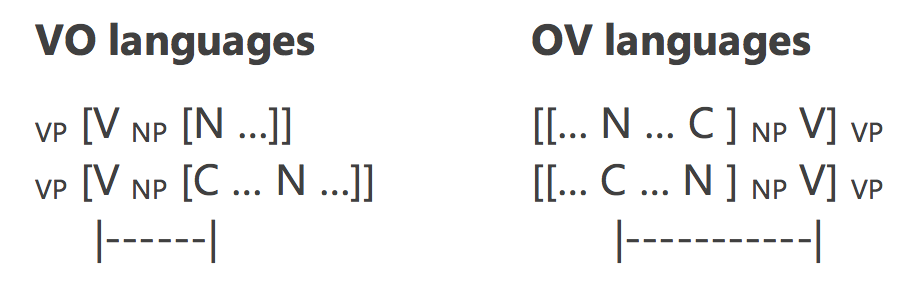
\includegraphics[width=\textwidth]{figures/Schmidtke-Bode_Figure 1.png}
\large
\begin{tabular}{l@{\hspace{2cm}}l}
\textbf{VO languages} & \textbf{OV languages} \\
\textsubscript{VP} [V \textsubscript{NP} [N ...]]       & [[... N ... C ] \textsubscript{NP} V] \textsubscript{VP}\\
\textsubscript{VP} [V \textsubscript{NP} [C ... N ...]] & [[... C ... N ] \textsubscript{NP} V] \textsubscript{VP}\\
\hphantom{\textsubscript{VP} [}|--{}--{}--{}--{}--{}|            & \hphantom{[[...}~~|--{}--{}--{}--{}--{}--{}--{}--| 
\end{tabular}
\end{figure}

From these considerations, one might derive the following prediction:

\eanoraggedright
{While all languages have source constructions for \isi{article}s (notably \isi{demonstrative}s for definite\is{definiteness} \isi{article}s and the \isi{numeral} ‘one’ for indefinite\is{definiteness} \isi{article}s), the \isi{grammaticalization} of these sources into more general NP markers should be a more productive historical process in VO languages than in OV languages. As a result, the synchronic typological distribution of \isi{article}s is significantly different in the two language types.}
\z
\noindent As a matter of fact, \citeapo{Hawkins2014_VarEff} prediction is narrower in scope: He applies it only to definite\is{definiteness} \isi{article}s, and only to independent definite\is{definiteness} \isi{article}s (i.e. words and clitics rather than affixes). The following examples illustrate the language types that are expected to be frequent according to \ref{ex:ksb:2}:

\ea\label{ex:ksb:2}
\ea  VO with definite\is{definiteness} \isi{article}\\
\langinfo{\ili{Maori}}{\ili{Austronesian}, \ili{Oceanic}}{\citealt{Bauer1993}: 256}\\
\gll I kite ia i te whare.\\
     \textsc{t/a}   see 3\textsc{sg}   \textsc{obj}   \textsc{det}   house\\
\glt ‘She saw the house.’

\ex
 OV without definite\is{definiteness} \isi{article}\\ 
\langinfo{\ili{Lezgian}}{Nakh-Daghestanian, Lezgic}{\citealt{Haspelmath1993}: 343}\\
\gll Ada-z  balk’an   aku-na.\\
     he-\textsc{dat}   horse     see-\textsc{aor}\\
\glt ‘He saw the horse.’
\z
\z\newpage
\noindent In support of the hypotheses in \REF{ex:ksb:2}, \iai{Hawkins} cites some of \citegen{Dryer2005_Def} \textit{WALS} data, which show, indeed, that free-standing definite\is{definiteness} \isi{article}s are relatively more frequent in VO-languages (more on the data below).

\iai{Hawkins}’s approach, as illustrated by this specific example, has a number of assets: For instance, it emphasizes the importance of the linear dimension of language, which tightly constrains production and parsing\is{processing} processes but which tended to be neglected by (at least early) \isi{cognitive}-linguistic and construction-based\is{Construction Grammar} approaches to grammar (see also \citealt{Diessel2011_Review} for a similar critique). \iai{Hawkins}’s work is clearly pioneering here, and in the recent usage-based\is{usage-based approach} literature, related notions like contextual \isi{predictability}, \isi{informativity} and projective links have come to take a highly prominent place (see, e.g., \citealt{GahlGarnsey2004,Levy2008_Exp,Auer2009_Online}). Furthermore, \iai{Hawkins}’s diachronic thinking adds a new dimension to classic research in \isi{grammaticalization}. As \citet[7]{Good2008_Intro} points out, work on \isi{grammaticalization} typically offers “permissive explanations […], that is, it focuses on particular \isi{grammaticalization} paths without, in general, accounting for what factors will cause one language, but not another, to instantiate those paths.” \iai{Hawkins}’s approach elevates this “permissive” nature of explanation to what Good (ibid.) calls a “probabilistic” one: It attempts to explain why certain \isi{grammaticalization} processes are set in motion only (or preferably) in certain language types or at certain points in time (see also \citealt{Hawkins1986_EngGer,Hawkins2012_Hist} for representative work along these lines).

But just how convincing are such claims and the empirical support that \iai{Hawkins} provides for them? In the present case, I have a number of reservations about the picture drawn in \citet{Hawkins2014_VarEff}.

To begin with, I do not quite see why the hypothesis is restricted to the development of definite\is{definiteness} \isi{article}s, as indefinite\is{definiteness} \isi{article}s should qualify equally well as NP constructors. Similarly, \iai{Hawkins}’s preoccupation with word-based \isi{processing} (which is prominent throughout his 2014 book), to the neglect of affixes with identical functions, is not sufficiently motivated. In addition to the problem that free and bound markers are very hard to distinguish consistently for cross-linguistic comparison \citep{Haspelmath2011_Word}, it remains unclear if there is a measurable \isi{psycholinguistic} difference between word- and affix-\isi{processing}. As long as there is no evidence for the view that free and bound \isi{definiteness} markers are parsed\is{processing} in fundamentally different ways, we should rather take a more embracing approach to the data and ask whether VO- and OV-languages differ in their propensity to grammaticalize\is{grammaticalization} \isi{article} morphemes from their respective source constructions.
\newpage
With these considerations in mind, the first step of the empirical assessment is, just like in \citet{Hawkins2014_VarEff}, to examine the typological distribution of \isi{article} morphemes. \iai{Dryer}’s \textit{WALS} data, in their most recent version, are set out in \tabref{tab:ksb:1}.


\begin{table}
\begin{tabularx}{.8\textwidth}{lYYYYl}
\lsptoprule
& VO &  OV &  ndo &  Totals\\
\midrule
Distinct ART word & 144 & 52 & 14 & 210 & \\
DEF affix & 49 & 33 & 6 & 88 & ART\\
DEM used as ART & 30 & 33 & 5 & 68 & \\
Only INDEF ART & 20 & 24 & 0 & 44 & \\
\midrule
No ART & 70 & 111 & 14 & 195 & NO ART\\
\midrule
\textbf{Totals} & \textbf{313} & \textbf{253} & \textbf{39} & \textbf{605} & \\
\lspbottomrule
\end{tabularx}
\caption{Distribution of articles in different word-order types (\citealt{Dryer2013_Def,Dryer2013_OV})}
\label{tab:ksb:1}
\end{table} 

For the purposes of testing our revised version of \iai{Hawkins}’s hypothesis, we need to discard the languages without a dominant order\is{word order} of V and O (“ndo”), and we basically conflate the figures in the first four rows of \tabref{tab:ksb:1} and contrast them with those in the final row. In other words, (i) we consider both free and bound \isi{definiteness} morphemes; (ii) we include those languages which are beginning to use a \isi{demonstrative} like an \isi{article} (row 3, see \citealt{Dryer2013_Def} for details) – thus incorporating cases of incipient \isi{grammaticalization}; (iii) we include languages with indefinite\is{definiteness} \isi{article}s only.\footnote{Some readers may object to this way of grouping the data. For example, one might reasonably argue that languages in which \isi{demonstrative}s are used with some \isi{article}-like functions should \textit{not} be said to have “proper” \isi{article}s (yet). However, even when such languages are classified differently for statistical purposes, the results remain the same in many respects (see supplementary material SM3.2).} The conflated form of the data thus looks like in \tabref{tab:ksb:2}.

\begin{table} 

\begin{tabularx}{.8\textwidth}{lYYY}
\lsptoprule
& VO  & OV & Totals\\
\midrule
ART morph & 243 & 142 & 385\\
No ART morph & 70 & 111 & 181\\
\midrule 
\textbf{Totals} & \textbf{313} & \textbf{253} & \textbf{566}\\
\lspbottomrule
\end{tabularx} 
\caption{Distribution of articles in different word-order types (reorganized)}
\label{tab:ksb:2}
\end{table} 

The distribution in \tabref{tab:ksb:2} looks conspicuously skewed, but of course these are raw data that are not controlled for genetic and areal effects.\footnote{For similar raw data, see also \citet{Dryer2009_Corr}, who endorses \iai{Hawkins}’s \isi{processing} explanation.} Therefore, what \iai{Hawkins}'s  (\citeyear{Hawkins2014_VarEff}) analysis clearly needs to be augmented with (in this case as well as virtually all others in his book) is proper statistical modelling according to contemporary standards (see, e.g., \citealt{Bickel2011_Modelling}). To this end, I am seeking converging evidence from two complementary quantitative approaches to the data, namely mixed-effects logistic regression\is{mixed-effects regression modelling} (see also \citealt{Cysouw2010_NP,JaegerEtAl2011}) and Bickel’s (\citeyear{Bickel2011_Modelling,Bickel2013_Fam}) \isi{Family Bias Method} (which is particularly suitable to testing hypotheses formulated in diachronic terms). In the supplementary materials to this paper\footnote{See \url{http://www.kschmidtkebode.de/publications} or \url{http://doi.org/10.5281/zenodo.2577480}.}, I offer a more detailed, non-technical introduction to the \isi{Family Bias Method} (SM1), as well as the statistical properties of all models (SM2–5). For reasons of space, I here confine myself to describing some major results of the analyses.\footnote{All statistical analyses were performed in \textit{R} 3.3.1 (\citealt{RTeam2016_R}). I am grateful to Taras Zakharko and Balthasar Bickel for making their Family Bias\is{Family Bias Method} algorithm freely available (\citealt{ZakharkoBickel2011}).}

\figref{fig:ksb:2} shows that there is a significant effect of \isi{word order} on the occurrence of \isi{article}s in a mixed-effects regression model\is{mixed-effects regression modelling} (\textit{β} = -0.73, \textit{p} < 0.001).\footnote{All regression analyses I performed are based on generalized linear mixed-effects models\is{mixed-effects regression modelling} that include genealogical and macro-areal dependencies as random effects (see SM3). The model in \figref{fig:ksb:2}, for example, contains by-family and by-area random intercepts for the distribution of \isi{article}s, while a by-area random slope for the word-order\is{word order} effect did not improve the model significantly and was hence excluded from the final model.} Although the model is not particularly good overall, probably missing important further predictors (\textit{R\textsuperscript{2}}\textit{\textsubscript{c}} = 0.14, \textit{C} = 0.72), \iai{Hawkins}’s hypothesized effect is clearly present, as the probability of \textit{not} having \isi{article}s (y-axis) increases significantly as we go from VO to OV (x-axis).

  

\begin{figure}
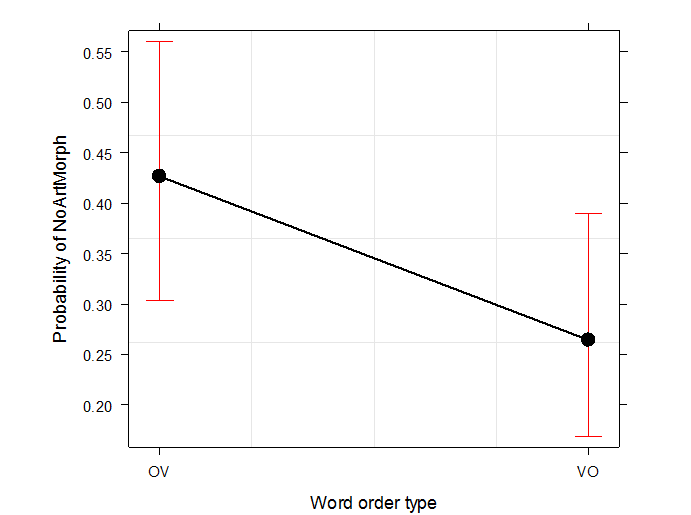
\includegraphics[height=.3\textheight]{figures/schmidtkebode-img2.png}
\caption{Effect of word order type on the probability of (not) having \isi{article}s in a mixed-effects model (see SM3 for details)}
\label{fig:ksb:2}
\end{figure}

In the Family Bias\is{Family Bias Method} estimations, too, it turns out that, among those families that do not just show a chance distribution of \isi{article}s, VO families are about 2.6 times more likely to develop \isi{article}s than OV families. This is illustrated in \tabref{tab:ksb:3}, and \figref{fig:ksb:3} shows that this effect is stable (i.e. never reversed) across all six macro areas. In sum, the global typological picture is consistent with \iai{Hawkins}’s \isi{processing} account, even when tested against a more comprehensive data set and with more rigorous modes of examination.
 

\begin{table}
\begin{tabularx}{.8\textwidth}{lYYY}
\lsptoprule
& VO &   OV &   Totals\\
\midrule 
ART morph & 50 & 19 & 69\\
No ART morph & 15 & 15 & 30\\
\midrule
\textbf{Totals} & \textbf{65} & \textbf{34} & \textbf{99}\\
\lspbottomrule
\end{tabularx} 
\caption{(Rounded) family biases for articles in different word-order types (N\textsubscript{total} = 217 genetic units, 99 of which are estimated to be “biased” (as opposed to internally diverse); Fisher exact test, \textit{p} = 0.039)}
\label{tab:ksb:3}
\end{table}
   
 
\begin{figure}
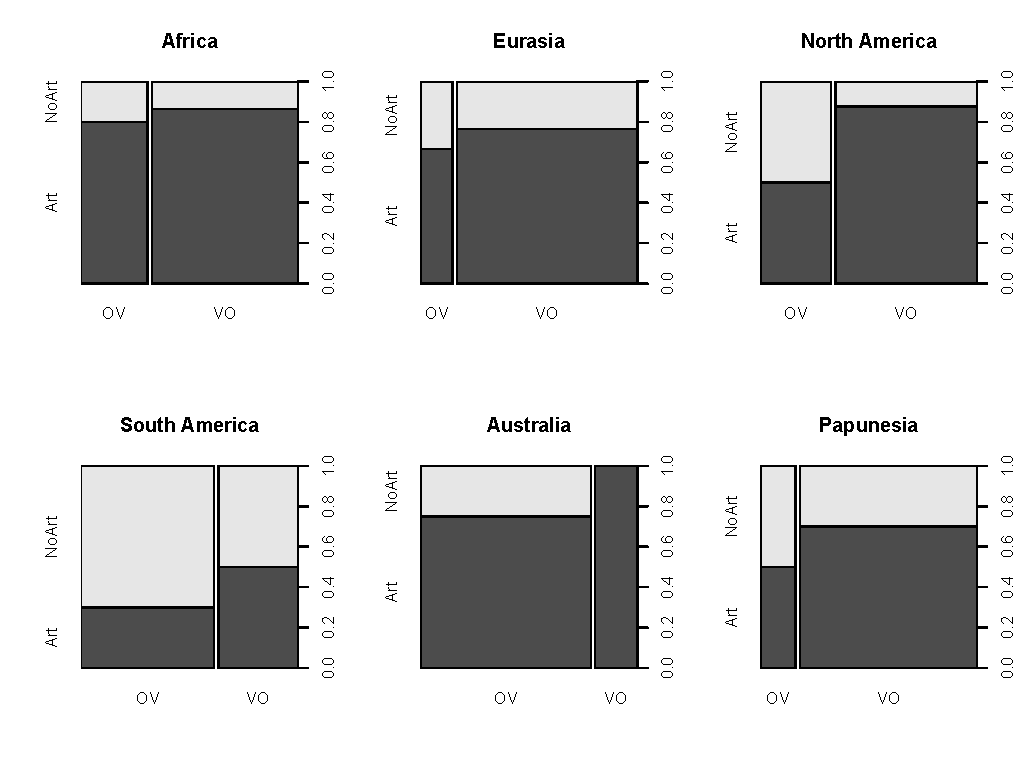
\includegraphics[width=\textwidth]{figures/ksb3.pdf}
\caption{Family biases by macro area (see SM2 for details)}
\label{fig:ksb:3}
\end{figure}
\newpage

Recall, however, that a second prediction of this account is that \isi{article}s are especially useful in those VO languages that have \isi{modifier}s before the head noun in NPs (\textit{a very delicious meal}). One would thus expect, for example, that the \isi{grammaticalization} of \isi{article}s is particularly productive in VO languages with ADJ\is{adjective}-N order, and, from an \isi{efficiency} perspective, less so in those with N-ADJ\is{adjective} order. I tested this by examining the order of nouns and \isi{adjective}s \citep{Dryer2013_Adj} in all VO languages in the same sample as above (N\textsubscript{total} = 278 languages). \newpage Across several different statistical models (and operationalizations of the hypothesis, see SM4), I did not find support for \iai{Hawkins}’s \isi{efficiency} hypothesis. In one analysis, for example, I probed whether free-standing \isi{article} words are more likely in VO languages with ADJ\is{adjective}-N order than in those with N-ADJ\is{adjective} order. \figref{fig:ksb:4} shows that this is neither the case for definite\is{definiteness} \isi{article}s nor for \isi{article}s in general.\footnote{Moreover, if we look at VO languages which are beginning to use a \isi{demonstrative} as a definite\is{definiteness} \isi{article} (N = 26 in \citealt{Dryer2013_Def}), \iai{Hawkins}’s account would lead us to expect that such incipient \isi{grammaticalization} is particularly frequent in the constellation DEM\is{demonstrative}-N and ADJ\is{adjective}-N (and again less frequent if N precedes both the ADJ\is{adjective} and the DEM\is{demonstrative}). Now, of the 26 languages in question, 22 are N-DEM and four are DEM-N. It is the latter type that is interesting here, and we find that two of these four languages are ADJ\is{adjective}-N and the other two N-ADJ\is{adjective}. Again, no clear pattern along Hawkinsian\ia{Hawkins} lines can be detected here.} 

  

\begin{figure}
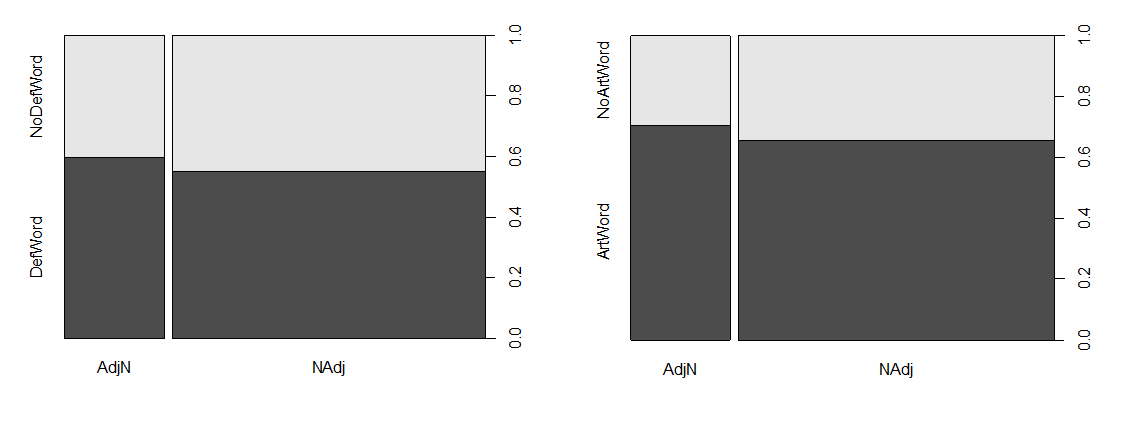
\includegraphics[width=\textwidth]{figures/schmidtkebode-img4.png}
\caption{Occurrence of articles in VO languages depending on the position of adjectives (left plot: definiteness words only; right plot: all \isi{article}-like words; for the corresponding mixed-effects models, see SM4)}
\label{fig:ksb:4}
\end{figure}

Clearly, this picture does not speak for a critical \isi{processing} pressure being at work. And the same conclusion actually carries over to OV languages: It is true that, to the extent that these languages show a reduced propensity for developing \isi{article}s, they manage to keep NP \isi{processing} domains slightly shorter; but there are several indications that this pressure cannot be particularly strong. 

First, our Family Bias\is{Family Bias Method} calculations show, in addition to the findings from above, that \textit{none} of the large OV families in the sample actually exhibits a significant bias (towards or against \isi{article}s) in the first place; they are all internally diverse, i.e. with no more than chance distributions of \isi{article}s (\tabref{tab:ksb:4}).\footnote{\citet{Bickel2013_Fam} suggests that the (minimum) strength of a universal pressure can be calculated on the basis of the proportion of biased families \textit{k} among all families of a particular kind \textit{n} (here: OV families): \textit{\^s}\textsubscript{} =\textsubscript{} (\textit{k}+1)/(\textit{n}+2). Based on the figures in \tabref{tab:ksb:4}, we obtain \textit{\^s}\textsubscript{(OV)} = (0+1)/(11+2) = 0.077. This estimate is so small in magnitude that one is forced to conclude that there is no particular pressure at all on OV languages with regard to the development of \isi{article}s.} 

\begin{table}
\begin{tabularx}{.8\textwidth}{lYYY}
\lsptoprule
& VO & OV &  Totals\\
\midrule
significantly biased & 12 & 0 & 12\\
internally diverse & 6 & 11 & 17\\
\midrule
\textbf{Totals} & \textbf{18} & \textbf{11} & \textbf{29}\\
\lspbottomrule
\end{tabularx}
\caption{Distribution of biases (for or against) articles among large families in the sample (N\textsubscript{total} = 29 genetic units)}
\label{tab:ksb:4}
\end{table}

Second, from a more qualitative perspective, there is suggestive evidence that a potential \isi{efficiency} motivation in OV languages is easily overridden by other factors. For example, \citet{Ross2001_Contact} discusses an interesting case of an intense \isi{contact} situation in which the \ili{Austronesian} language \ili{Takia} adapted\is{adaptation} its VO syntax to the OV structure of its Papuan \isi{contact} language \ili{Waskia}. Ross argues that, in the wake of this restructuring, \ili{Takia} speakers must have shed the prenominal \isi{article} word in NPs (see \ref{ex:ksb:4}a), which would be fully in line with \iai{Hawkins}’s prediction. At the same time, however, the degree of linguistic \isi{accommodation} was so intense that \ili{Takia} speakers also did something else: They grammaticalized\is{grammaticalization} a postnominal deictic\is{deixis} element into a postnominal \isi{demonstrative} with some \isi{article}-like functions, reproducing exactly the \isi{article} pattern in \ili{Waskia} (see \ref{ex:ksb:4}b-c).

\ea\label{ex:ksb:4} 
  \ea
  \langinfo{Proto-Western \ili{Oceanic}}{}{\citealt[142]{Ross2001_Contact}}\\
  \gll \textbf{a}   tam\textsuperscript{w}ata   a-ña\\
      \textbf{\textsc{det}}   man   that-3\textsc{sg}\\
  \glt ‘that man’

  \ex 
  \langinfo{\ili{Takia}}{\ili{Austronesian}, \ili{Oceanic}}{\citealt{Ross2001_Contact}: 140}\\
  \gll \ili{Waskia}   tamol  \textbf{an}\\
      Waskian   man   \textbf{that}\\
  \glt ‘that \ili{Waskia} man’

  \ex
  \langinfo{\ili{Waskia}}{Nuclear Trans New Guinea, Madang}{\citealt{Ross2001_Contact}: 140}\\
  \gll \ili{Waskia}   kadi   \textbf{mu}\\
      \ili{Waskia}   man   \textbf{that}\\
  \glt ‘that \ili{Waskia} man’
  \z
\z

In other words, \ili{Takia} speakers chose precisely the diachronic route that \iai{Hawkins} would predict to be disfavoured, which goes to show that the alleged \isi{processing} pressure cannot have been very strong, after all. In this connection, one may also recall that our regression\is{mixed-effects regression modelling} model from above, while bringing out a significant global effect from \isi{word order} type, did not provide a particularly good fit to the data. The substantial amount of variation in the data that it cannot account for must thus be attributed to other, possibly stronger factors.\footnote{Diachronic research has actually put forward a number of plausible candidates for such factors. A prominent one since at least \citet{Vennemann1975_Drift} is the loss of a \isi{case} system and the concomitant rigidification of constituent order\is{word order}, which favours the development of \isi{article}s to express information-structural\is{information structure} distinctions that were previously coded by a more flexible \isi{word order} (see also \citealt{Hawkins2004_Eff,HewsonBubenik2006,Fischer2010_WOChange,CarlierLamiroy2014}). Another possible factor is the loss of an aspectual\is{aspect} system (\citealt{Abraham1997_Asp,Leiss2000_Asp,Leiss2007_Def}). However, especially the former type of explanation is often viewed critically (e.g. \citealt{Selig1992_LatDet} on \ili{Romance}; \citealt{McCollMillar2000_Def} on \ili{English}; \citealt{Leiss2000_Asp} on \ili{Germanic}), and there is currently no proposal as to how various factors may conspire to explain the synchronic distribution of \isi{article}s (see also \citealt{Lüdtke1991}). For some further information and preliminary typological analyses of these factors, interested readers are kindly referred to SM5.}

We conclude, then, that \citet{Hawkins2014_VarEff} correctly predicts a global difference between OV- and VO-languages in the development of \isi{article}s. But the present analysis also revealed some challenges for this account. Therefore, it still needs to be established by future research whether the global correlation between \isi{word order} type and the absence of \isi{article}s really reflects a \textit{causal} connection between these two phenomena, and whether this could be attributed to efficient\is{efficiency} information \isi{processing}. If it turns out that \iai{Hawkins} is correct, the findings in the present section suggest that we would be dealing with a ‘weak universal pressure’ in the sense of \citetv{Seržant2019tv} or a “weak cognitive bias” with “significant population-level consequences” (\citealt{ThompsonEtAl2016}: 4530).

\section{Concluding remarks} 

The present contribution has taken a closer look at John \iai{Hawkins}’s “\isi{processing} typology”, a research programme that fully subscribes to functional-adaptive\is{adaptation} motivations for grammatical structure. In the first part of the paper, I discussed where such motivations are possibly operative in diachronic change. In my view, a case can be made for \iai{Hawkins}’s \isi{efficiency} considerations in the process of \isi{actualization}, i.e. when a linguistic \isi{innovation} comes to be extended to a principled, cross-linguistically similar subset of potential application sites (as in differential \isi{flagging} and indexing\is{indexation}, relativization\is{relative clause}, etc.). In this respect, I consider \iai{Hawkins}’s account as superior to purely source-oriented explanations of grammatical patterns. Of course, this does not deny that \isi{persistence} accounts are relevant to typological patterns – they clearly are; but it argues against \isi{persistence} as the sole or perhaps even the dominant explanatory principle for grammatical universals.

A more ambitious but also undoubtedly more problematic move is to link parsing\is{processing} and \isi{efficiency} to certain \isi{innovation} processes, such as when a particular \isi{grammaticalization} channel is predicted to be set in motion only under specific structural conditions. In the brief case study presented here, we saw that \iai{Hawkins}’s NP \isi{processing} hypothesis provides a neat match to the global typological data, even when these are analyzed in more rigorous and hence more appropriate ways than in \citet{Hawkins2014_VarEff}. On the other hand, the details of neither the typological picture nor individual diachronic studies produce evidence for a strong pressure on languages to develop into the predicted directions. Therefore, the hypothesis that speakers of OV languages are significantly less inclined than speakers of VO languages to grammaticalize additional NP constructors, remains plausible but currently rather weakly substantiated. 
\newpage
What we would need to see to make it more convincing is a triangulation of (i) typological data that are large enough to take several alternative predictor variables from the literature into account (e.g. \isi{case} and \isi{aspect} systems, the presence of other NP constructors such as \isi{classifier}s), (ii) diachronic data from languages that have undergone (or are in the process of undergoing) changes in basic \isi{word order}, (iii) behavioural evidence, such as \isi{psycholinguistic} experimentation with \isi{artificial language}s (e.g. along the lines of \citealt{CulbertsonEtAl2012}; see also \citealtv{Levshina2019tv}). As a matter of fact, a particularly strong aspect of \iai{Hawkins}’s work (especially in \citealt{Hawkins2004_Eff,Hawkins2014_VarEff}) is that it generally attempts precisely this kind of methodological cross-fertilization; but for the domain at issue here, such an approach has yet to be fleshed out in sufficient detail.

\section*{Abbreviations}

The paper follows the Leipzig Glossing Rules. Additional abbreviation: T/A = \isi{tense}/\isi{aspect} marker

\section*{Acknowledgements}

The research for this paper was carried out in the context of the project \textit{Form-\isi{frequency} correspondences in grammar} at Leipzig University. The support of the European Research Council (ERC Advanced Grant 670985, Grammatical Universals) is gratefully acknowledged. I would like to thank John \iai{Hawkins}, Mark Dingemanse, the co-editors of the present volume as well as the audiences of the Diversity Linguistics Conference (Leipzig,  {March 2017}), the 3\textsuperscript{rd} Usage-Based Linguistics Conference (Jerusalem,  {July 2017}) and the Syntax of the World’s Languages VIII Conference (Paris,  {September 2018}) for very helpful feedback on previous versions of this paper. The usual disclaimers apply.

\sloppy
\printbibliography[heading=subbibliography,notkeyword=this] 
\end{document}